Here we test our Genetic Allocator directly in the out of sample period. We decided to set the parameters for the Fitness function as explained in the relative section. We then used a backward-looking window to compute the sharpe ratio of each portfolio during the optimization of 60 days.\\
We then let the algorithm work on its own and after a couple of hours of optimization the optimal portfolio yields the following results:

\begin{table}
	\centering
	\begin{tabular}{c|c}
		\textbf{Statistic} & \textbf{Value} \\\hline
		Sharpe Ratio & 4.9597 \\ 
		Sortino Ratio & 6.761 \\ 
		Omega Ratio & 2.83 \\ 
		Skewness & 2.9578  \\ 
		Kurtosis & 51.4854 \\ 
		Maximum Drawdown (\% duration/duration) & 9.4 \\ 
		Longest Drawdown (days) & 136 \\ 
		Winning Days & 66.5975 \\ 
	\end{tabular}
	\caption{\label{tab:gentic_OOS} Statistics for the out-of-sample performance of the Genetic Portfolio algorithm.}
\end{table}


\begin{center}
	\centering
	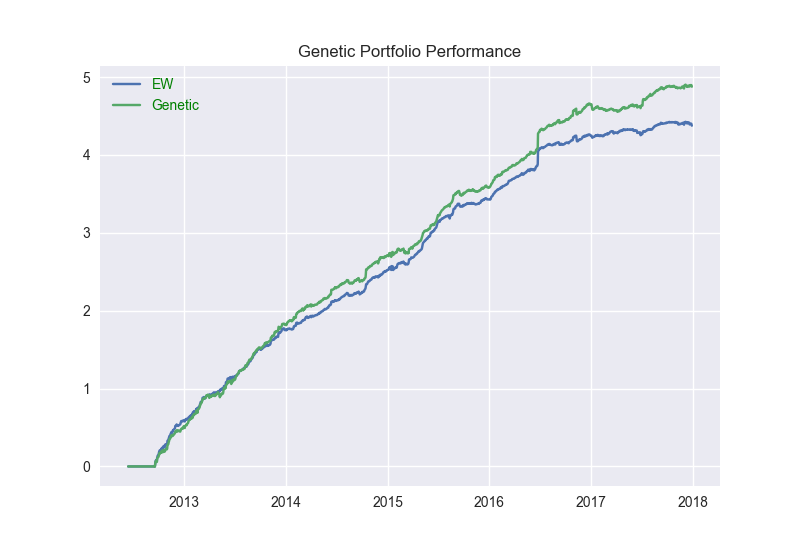
\includegraphics[width=0.6\textwidth]{Genetic_Algo/Try_1_oos.png}
	\captionof{figure}{Out-of-Sample equity line of the Genetic Portfolio algorithm.}
	\label{Genetic_Line}
\end{center}

\begin{center}
	\centering
	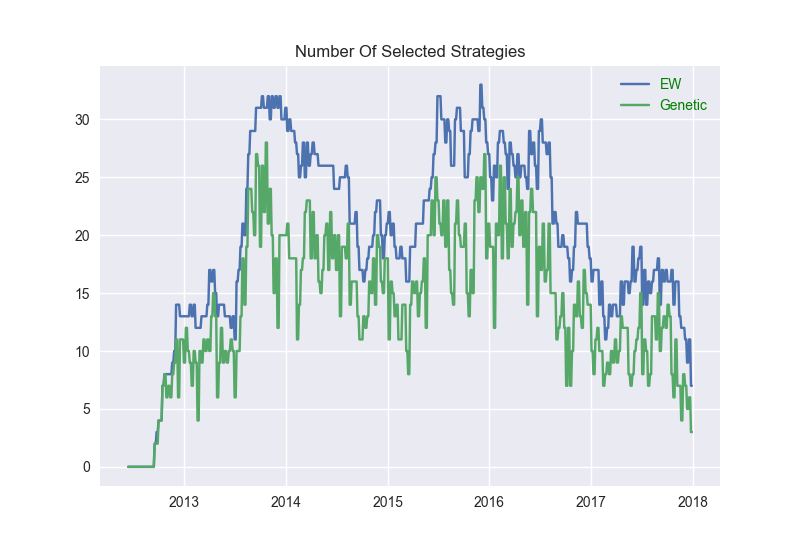
\includegraphics[width=0.6\textwidth]{Genetic_Algo/Try_1_num_strats.png}
	\captionof{figure}{Number of strategies selected out-of-sample from the Genetic Portfolio algorithm.}
	\label{Genetic_num_strats}
\end{center}

The equity line can be found in figure \ref{Genetic_Line}, and the number of selected strategies can be found in \ref{Genetic_num_strats} .
In the end the method performs in some aspects better than the equally weighted portfolio, but still the performance is not exceptional as we hoped initially. Both the Sharpe-Ratio and the Sortino-Ratio of this portfolio do not manage to be better than an equally weighted portfolio. In the end, the PnL is a bit higher, but this comes at a higher risk that is not what we are looking for. We have to sadly set this method apart and focus our attention once again on simpler and more intuitive models. The major drawback of this Genetic Learner is that despite being very interesting and potentially powerful it leaves little possibility to understand the underlying optimization process and to control it. We will now move forward towards an alternative method.